\documentclass[letter, 10pts]{article}
\usepackage[monocolor]{../math232/ahsansabit}
\usepackage[]{float}
\usepackage{tikz}
\usepackage{tikz-3dplot}
\usepackage[outline]{contour} % glow around text
\usepackage{xcolor}
\usepackage{pdfpages}
\usepackage[]{pgfplots}\usepackage{physics}
\usepackage{multicol}
\colorlet{veccol}{green!50!black}
\colorlet{projcol}{blue!70!black}
\colorlet{myblue}{blue!80!black}
\colorlet{myred}{red!90!black}
\colorlet{mydarkblue}{blue!50!black}
\tikzset{>=latex} % for LaTeX arrow head
\tikzstyle{proj}=[projcol!80,line width=0.08] %very thin
\tikzstyle{area}=[draw=veccol,fill=veccol!80,fill opacity=0.6]
\tikzstyle{vector}=[-stealth,myblue,thick,line cap=round]
\tikzstyle{unit vector}=[->,veccol,thick,line cap=round]
\tikzstyle{dark unit vector}=[unit vector,veccol!70!black]
\usetikzlibrary{angles,quotes} % for pic (angle labels)
\contourlength{1.3pt}
\title{Classical Mechanics : : Homework 07}
\author{Ahmed Saad Sabit, Rice University}
\date{\today}
\newcommand{\hb}{\hbar}
\newcommand{\U}{\uparrow}
\newcommand{\D}{\downarrow}
\usepackage[]{braket}
\begin{document}
\maketitle
\section*{Problem from Previous problem set}
\subsection*{(a)} 
\begin{align*}
	A[y] &= \int_{-a}^{a} y(x) \, \mathrm{d} x  \\
	S(y) &= \int_{-a}^{a} \sqrt{1 + y'^2}  \, \mathrm{d} x = 2L 	
\end{align*}
Required maximization 
\[
	\text{max}\left(A[y]\right) = \int_{-a}^{a}  y(x)  - \lambda \sqrt{1 + y'^2} \, \mathrm{d} x \implies \text{treat integrand as Lagrangian}
\] 
Setting euler lagrange equation 
\[
\frac{\mathrm{d} }{\mathrm{d} x} \left(\frac{y'}{\sqrt{1 + y'^2}  } \right) = \frac{1}{\lambda}
\] 
Using online integral calculator I receive with substitution $u = y'$ 
\[
\frac{u}{\sqrt{1 + u^2} } = - \frac{x}{\lambda} + C
\] 
\begin{align*}
	u = y ' &= \sinh \left(\frac{x}{\lambda} - k\right) \\ 
	y(x) &= - \lambda \cosh \left( \frac{x}{\lambda} - k \right) + C
\end{align*}
Hence length constraint 
\begin{align*}
	2 L = \int_{-a}^{a} \sqrt{1 + y'(x)^2}  \, \mathrm{d} x = 2 \lambda \sinh \left(\frac{a}{\lambda}\right)
	\\
	L &= \lambda \sinh \left(\frac{a}{\lambda}\right) \\
	\frac{L}{\lambda} &= \sinh \left(\frac{a}{\lambda}\right) \\
\end{align*}
 
Using length constraint we now solve for $y(x)$ for this problems (eliminate $C$) as $y = 0$ for $x = \pm a$
\[
y(x) = \lambda 
\left(
\cosh \left(a / \lambda \right) - 
\cosh \left(x / \lambda\right)
\right)
\] 

\subsection*{(b)} 
\begin{figure}[H]
	\centering
	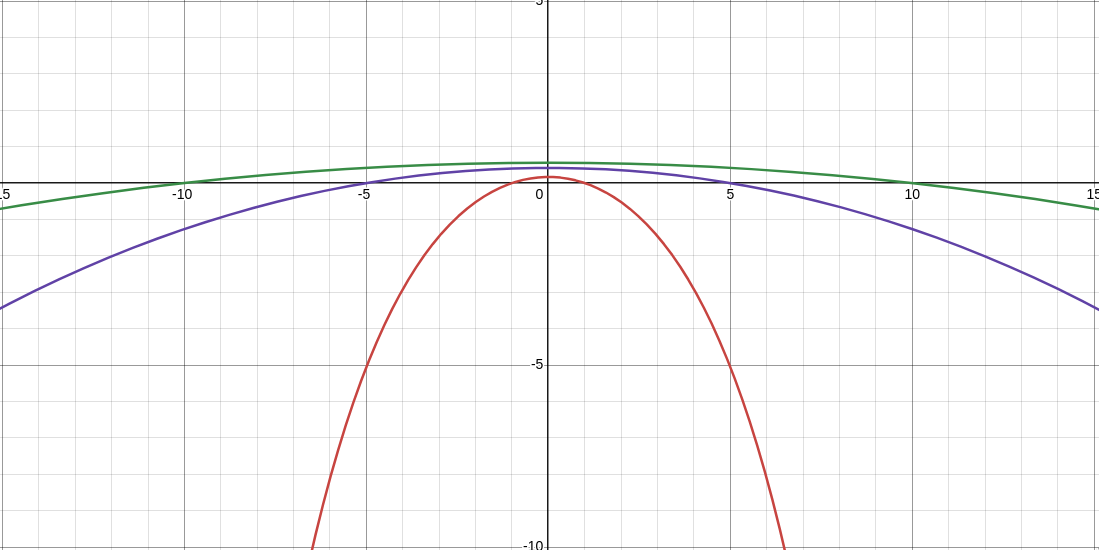
\includegraphics[width=0.8\textwidth]{ss/7/2.png}
	\caption{For various $a$ values we plot the rough diagram [this is not exact because of trancendental behavior].}
	\label{fig:ss-7-2-png}
\end{figure}

\subsection*{(c)} 
\begin{align*}
	A &= \int_{-a}^{a} y(x) \, \mathrm{d} x 
\\
&= \int_{-a}^{a}  \lambda 
\left(\cosh (a / \lambda) - \cosh ( x / \lambda )\right) \,\mathrm{d} x \\
&= 2 a \lambda \cosh(a / \lambda) - 2 \lambda ^2 \sinh ( a / \lambda ) \\
\end{align*}
Maximization happens at $ a / \lambda = \tanh ( a / \lambda ) $ and $a / \lambda$ is numerically $1.2$. Using that and putting it together with length of this system 
\[
a = \frac{1.2}{L} \sinh \left(\frac{a^2}{1.2}\right)
\] 

\section*{Problem 1}
\subsection*{(a)} 
We will do the computation with the assumption that the particle will not leave the surface of the wedge, by which I mean we avoid jumping behavior for now. 

We can observe that in the problem $x,l$ can safely be our generalized coordinates $(q_1(t), q_2(t) ) = (x(t), l(t))$. I have done some scratch work on the attached appendix to validate this. 

Let's imply constraints from the start and write each coordinate equations. 

Hence position of the top corner of the wedge
\[
	(x_1, y_1) = (x_1, H) = (q_1, H) \implies (x(t), H)
\]

Position of the ball
\[
	(x_2, y_2) = (l(t) \cos \alpha + x(t), H - l(t) \sin \alpha )
\]

For convenience let's set our origin to be at $(0, H)$ instead of $(0,0)$ in the figure. Then 
\begin{align*} 
	(x_1, y_1) &= (x(t), 0) \\ 
	(x_2, y_2) &= (l(t) \cos \alpha + x(t),  - l(t) \sin \alpha )
\end{align*}
Respective velocity is then, 
\begin{align*} 
	(\dot x_1,  \dot y_1) &= ( \dot x(t), 0) \\ 
	(\dot x_2, \dot y_2) &= (\dot l(t) \cos \alpha + \dot x(t),  - \dot l(t) \sin \alpha )
\end{align*}

The respective speed squared is
\begin{align*} 
	|(\dot x_1,  \dot y_1)|^2 &= \dot x(t) ^2 \\ 
|	(\dot x_2, \dot y_2) |^2&= 
\dot l(t) ^2  \cos ^2 \alpha + \dot x(t) ^2 + 2 \dot x(t) \dot l(t) \cos \alpha  + \dot l(t) ^2 \sin ^2 \alpha  \\ 
&=  
\dot l(t) ^2   + \dot x(t) ^2 + 2 \dot x(t) \dot l(t) \cos \alpha   
\end{align*}

Now to compute lagrangian we need the individual energy. Let's write the kinetic and potential energy (setting $y = 0$ in our new coordinate system at $U_g = 0$ gravitational potential energy)
\begin{align*}
	K_\text{total} &= \frac{1}{2}M \dot x(t)^2 + 
	\frac{1}{2} m \left(\dot l (t) ^2 + \dot x (t) ^2  + 2 \dot x(t) \dot l(t) \cos \alpha \right)\\
U_\text{total} &=  	
	U_\text{spring} (x(t)) + 
	U_\text{gravity} (l(t)) = \frac{1}{2} k (x(t) - x_0)^2 
	- m g l(t) \sin \alpha\\ 
	\implies \mathcal L &= 
\frac{1}{2} (M + m ) \dot x (t) ^2 + 
\frac{1}{2} m \dot l (t) ^2 + 
m \cos \alpha \dot x(t) \dot l(t)  
- \frac{1}{2} k (x(t) - x_0)^2 + mg \sin \alpha 	 l(t)
	\\
\end{align*}

The Euler Lagrange Equation here is 
\[
	\frac{\mathrm{d} }{\mathrm{d} t} 
	\frac{\partial \mathcal L}{\partial \dot q_i} = 
	\frac{\partial \mathcal L }{ \partial q_i }
\] 
\begin{align*}
	\frac{\mathrm{d} }{\mathrm{d} t 
	}
	\frac{\partial \mathcal L}{\partial \dot x} 
	&= 
	(M+m) \ddot{x}(t) + 
	m \cos \alpha \ddot{l}(t) 
	\\
	\frac{\mathrm{d} }{\mathrm{d} t 
	}
	\frac{\partial \mathcal L}{\partial \dot l} 
	&= 
	m \ddot{l}(t) + m \cos \alpha \ddot{x}(t) 
	\\
	\frac{\partial \mathcal L}{\partial x} &= 
        -k (x(t) - x_0) 
	\\
	\frac{\partial \mathcal L}{\partial l} &= 
	mg \sin \alpha 
\end{align*}
The system of equations we get are then 
\begin{align*}
	(m + M) \ddot{x} (t) + m \cos \alpha \ddot{l}(t) &= - k (x(t) - x_0) \\
	m \cos \alpha \ddot{x}(t) + m \ddot{l}(t) &= mg \sin \alpha  \\
\end{align*}

I use the assistance of mathematica to find the solution with the very obvious bound cases 
\begin{align*}
	x(t) &= x_0 + \frac{mg \sin \alpha \cos \alpha}{k} 
	\left(\cos 
	\left(t\sqrt{\frac{k}{m \sin ^2 \alpha + M} }   \right) - 1\right)\\
	l(t) &= \frac{g \sin \alpha }{2} t^2 + 
	\frac{mg \sin \alpha \cos ^2 \alpha}{k} 
	\left(1-
\cos \left(
t \sqrt{\frac{k}{m \sin ^2 \alpha + M}} 
\right)
	\right)\\
\end{align*}

\subsection*{(b)} 
For a fixed wedge the solution is the obvious $l(t) = \frac{g \sin \alpha}{2}t^2$ and $\cos (t)$ never being greater than 1 causing $l(t)$ for the oscillating wedge is at slowest possible equal to $g \frac{\sin \alpha}{2} t^2$ which is the equation for the fixed wedge. 

At fastest case we have $l(t) = g \sin \alpha (\frac{1}{2}) t^2 + \frac{2 mg \sin \alpha \cos ^2 \alpha  }{k}$ thus oscillating $l(t)$ being greater than fixed $l(t)$ leaves us with the conclusion that  \emph{particle reaches the bottom faster for oscillating wedge.}
\begin{figure}[H]
	\centering
	\begin{tikzpicture}
		\begin{axis}[
			xmin= -10, xmax= 10,
			ymin= -10, ymax = 10,
			axis lines = middle,
		]
			\addplot[domain=-10:10, samples=100, color = cyan]{0.5*x*x + 199 * (1 - cos(2*x))};
			\addplot[domain=-10:10, samples=100]{0.5*x*x};
		\end{axis}
	\end{tikzpicture}
	\caption{The parabolic solution of $l(t)$ with respect to $t$ time for fixed wedge case in solid black. With the actual plot with $\cos f(t)$ term in cyan.}
	\label{}
\end{figure}

\section*{Problem 02} 
\subsection*{(a)} 
\emph{Final answer for grader: there are TWO degrees of freedom. BUT, if $h(t)$ is being controlled manually then ONE.}
\[
	(q_1,q_2) = (q_1(t), q_2(t)) = (x(t) , h(t))
\]  
\textbf{Free case:} There in total 3 masses. They are constrained in 2 dimensions that can be explained by $\mathbb{R}^{2}$.So there in total $2*3 = 6$ possible coordinates to explain the position of the system. This is without computing constraints. 

\textbf{Constraints: }Now taking account of constraints 
\begin{itemize}
	\item First mass is constrained vertically.
	\item Second mass is constrained horizontally. 
	\item First and Second mass have fixed distance constraint.
	\item Third mass is constrained along the line of the other two masses with a spring. 
	\item \textbf{If}, $h(t)$ is controlled by external driver, then this adds to the constraint.  
\end{itemize}
Each 4 constraints give us 4 equations. For illustrative and aesthetic purposes I note them here with the problem written in terms of the two generalized coordinate we'd pick.

\textbf{Generalized Coordinate:} $6 - 4$ free subtracted by constraints give us $2$ hence we just need two coordinate to explain this system. We will pick the vertical position of the first mass $y_1 = h(t)$ and position of third mass along the line of $1-3$ given by $(x_3, y_3) = \vec{f}(x(t))$ as our generalized coordinate. 

Note that our basis is the cartesian basis here. 

\begin{align*}
	(x_1, y_1) &= (0, h(t)) \\
	(x_2, y_2) &= (x_2(t), 0 ) = \underbrace{(\sqrt{R^2 - h^2(t)} , 0)}_{\text{using third constraint}} \\
R &=  	\text{Distance}[(x_1,y_1),(x_2,y_2)] \\
	(x_3, y_3) &= \left(x(t) \frac{\sqrt{R^2 - h^2(t) }  }{R} , h(t) - x(t) \frac{h(t)}{R}\right)  \\
\end{align*}

The fourth equation above can be solved by using similar triangle that gives us the two ratios (or you can just use Trigonometry to do it, I didn't want to see the face of sin cos tan in this problem because it is not the generalized coordinate but it doesn't really matter) 

\begin{align*}
	\frac{\sqrt{R^2 - h^2(t) } }{R} &= \frac{x_3}{x} \\
	\frac{h(t)}{R} &= \frac{h(t) - y_3}{x}
	\tag{For particle three constraint} 
\end{align*}
Now if there is an external driving force, then 
\[
y_1 = h(t) = F(t)	
\]
Where $F(t)$ is some known value caused by the driver.  If we consider this given drive then we have one more constraint that leaves us with $x(t)$ being the only generalized coordinate.  






\subsection*{(b)} 
Solve for the individual velocities first
\begin{align*}
	v_1 = (\dot x_1, \dot y_1) &= \dot h(t) \\
	v_2 = (\dot x_2, \dot y_2) &= - \dot h(t) \frac{h(t)}{\sqrt{R^2 - h^2(t)}}  \\
v_3 = 	\text{magnitude}(\dot x_3, \dot y_3) &=
\frac{\mathrm{d} }{\mathrm{d} t}
\left(x(t) \frac{\sqrt{R^2 - h^2(t) }  }{R} , h(t) - x(t) \frac{h(t)}{R}\right)  
\\&= 
\left(
\dot x(t) \frac{\sqrt{R^2 - h^2(t) }  }{ R} -
\dot h(t) \frac{x(t) h(t) }{R \sqrt{R^2 - h^2 (t )} }, 
\dot h(t) (1 - x(t) / R) - \dot x(t) h(t) / R
	\right)
\\
v_3^2 &\implies 
\left(
	\dot x(t) \frac{\sqrt{R^2 - h^2(t) }  }{ R} -
	\dot h(t) \frac{x(t) h(t) }{R \sqrt{R^2 - h^2 (t )} }
\right)^2 + 
\left(
	\dot h(t) \left(1 - \frac{x(t)}{R} \right) - \dot x(t) \frac{h(t)}{R}
\right)^2
\end{align*}
Write the kinetic and potential energy individually. I hate spending brain to trying to keep equations short enough. I did not want to do a trigonometric substitution for $h(t) = R \cos \alpha(t)$ to avoid transformation but it's going to cost me this huge equation no matter what. Whatever we will stick with what we are doing.  

We will gauge the horizon $y = 0$ as $U_g(y = 0) = 0$
\begin{align*}
	T_\text{tot}  - U_\text{tot}&= 
\frac{1}{2} m_1 v_1^2 + 
\frac{1}{2} m_2 v_2^2 + 
\frac{1}{2} m_3 v_3^2 - U_\text{spring} - U_\text{grav}
	\\ \mathcal L 
		     &=	\frac{1}{2} m_1 \dot h^2(t) + 
	\frac{1}{2} m_2 \dot h^2(t) \frac{h^2(t)}{R^2 - h^2 (t)} +  \\ &
+ 	\frac{1}{2} m_3 
	\left(
\left(
	\dot x(t) \frac{\sqrt{R^2 - h^2(t) }  }{ R} -
	\dot h(t) \frac{x(t) h(t) }{R \sqrt{R^2 - h^2 (t )} }
\right)^2 + 
\left(
	\dot h(t) \left(1 - \frac{x(t)}{R} \right) - \dot x(t) \frac{h(t)}{R}
\right)^2
	\right) \\ 
& - \frac{1}{2} k (x(t) - x_0)^2 - m_1 g h(t) - m_3 g h(t) \left(1 - \frac{x(t)}{ R} \right)
\end{align*}

The lagrangian is 
\begin{align*}
	 \mathcal L 
		     &=	\frac{1}{2} m_1 \dot h^2(t) + 
	\frac{1}{2} m_2 \dot h^2(t) \frac{h^2(t)}{R^2 - h^2 (t)} +  \\ &
+ 	\frac{1}{2} m_3 
	\left(
\left(
	\dot x(t) \frac{\sqrt{R^2 - h^2(t) }  }{ R} -
	\dot h(t) \frac{x(t) h(t) }{R \sqrt{R^2 - h^2 (t )} }
\right)^2 + 
\left(
	\dot h(t) \left(1 - \frac{x(t)}{R} \right) - \dot x(t) \frac{h(t)}{R}
\right)^2
	\right) \\ 
& - \frac{1}{2} k (x(t) - x_0)^2 - m_1 g h(t) - m_3 g h(t) \left(1 - \frac{x(t)}{ R} \right)
\end{align*}

\begin{comment} 
\rotatebox{-45}{$
	 \mathcal L 
		     = 	\dfrac{1}{2} m_1 \dot h^2(t) + 
	\frac{1}{2} m_2 \dot h^2(t) \dfrac{h^2(t)}{R^2 - h^2 (t)} +  
+ 	\frac{1}{2} m_3 
	\left(
\left(
	\dot x(t) \frac{\sqrt{R^2 - h^2(t) }  }{ R} -
	\dot h(t) \frac{x(t) h(t) }{R \sqrt{R^2 - h^2 (t )} }
\right)^2 + 
\left(
	\dot h(t) \left(1 - \frac{x(t)}{R} \right) - \dot x(t) \frac{h(t)}{R}
\right)
	\right) ^2
 - \frac{1}{2} k (x(t) - x_0)^2 - m_1 g h(t) - m_3 g h(t) \left(1 - \frac{x(t)}{ R} \right)
$}
\end{comment} 
It's okay if our $m_1, m_2$ are unknown because they are not coefficients of any function or variation of $x(t)$. So taking Lagrangian derivative they vanish. 

\textbf{NOTE:} 
This same equation can be solved to be NOT a function of $m_1, m_2$ because they are not coefficients of $x(t)$ hence get deleted while the derivatives are taken for EL Equations. A more digestable form of the exact same equation above after cutting of $m_1,m_2$ terms and doing further algebra is 
\[
\mathcal L 
=
\frac{1}{2} m 
\left(
\dot x ^2  
+ 
\dot h ^2 
+ 
\frac{x^2 h^2 \dot h ^2}{R^2 (R^2 - h^2) } 
- 
\frac{2 \dot x h \dot h + 2 x \dot h ^2}{R}
+ 
\frac{x^2 \dot h ^2}{R^2}	
\right) 
- 
\frac{1}{2}k (x - x_0)^2 - mgh (1 - x / R)
\] 

\subsection*{(c)}
Here we will consider $h(t)$ is known. Then we only require to understand the $x(t)$ equation of motion.
\begin{figure}[H]
	\centering
	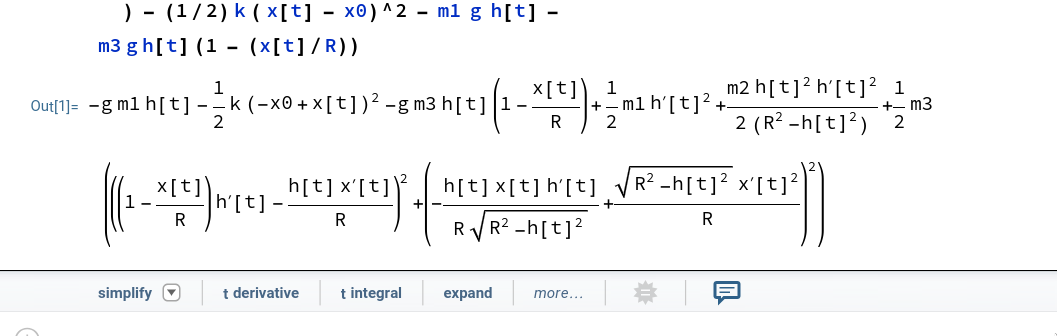
\includegraphics[width=0.8\textwidth]{ss/7/1.png}
	\caption{The output here is the Lagrangian. }
	\label{fig:ss-7-1-png}
\end{figure}

I do the EL equation in mathematica that leaves me with 
\[
\ddot{x} + x
\left(
\frac{k}{m} 
- 
\frac{\dot h ^2}{R^2} - 
\frac{h^2 \dot h ^2}{R^2 (R^2 - h^2)}
\right) =
\frac{\dot h ^2 + h \ddot{h} }{R} + \frac{gh}{R} + \frac{k}{m} x_0
\] 
Now if I define and write the obvious solution
\begin{align*}
	\tilde{A} &= \frac{k}{m} - \frac{\dot h(t) ^2}{R^2} - \frac{h(t)^2 \dot{h}(t)^2}{R^2 ( R^2 - h^2)} \\  
	\tilde{B} &= \frac{\dot h(t)^2 + h(t) \ddot{h}(t ) }{R} + \frac{g h(t) }{R} + \frac{kx_0}{m} \\
x(t) &= 
\frac{1}{\tilde{A}} 
\left(
\tilde B 
\left[ 
1 - \cos \left(t\sqrt{ \tilde A} \right)
\right]
+ 
\tilde A x_0
 \cos \left(t\sqrt{ \tilde A} \right)
\right)
\\
\end{align*}


\subsection*{(d)} 
\begin{align*}
	H &= \frac{\partial \mathcal L}{\partial \dot x} - \mathcal L \\ 
	&=  \text{Plugged in the formula of Lagrangian and it's derivative wrt. speed} \\ 
	&=  \text{and doing further simplification, attached in handwritten appendix}\\
	&= \frac{1}{2} m \dot x ^2 - 
	\frac{1}{2} m 
	\left(
\dot h ^2 + \frac{x^2 \dot h ^2}{R^2 - h^2} - 2 \frac{x \dot h^2 }{R}
	\right) + 2 gh \left( 1 - x / R\right) + \frac{1}{2} k (x - x_0)^2\\
\end{align*}
Hamiltonian is equal to total energy because we have a normal form of Generalized Potential that only depends on generalized coordinate (not its derivative) and also not depends on time. And this function not being a function of time stays constant as time progresses. 


\subsection*{(e)}
If we plug in $h(t) = R \cos( \omega t)$ and using wolfram I get
\begin{align*}
	\tilde A &=  \frac{k}{m} - \omega^2 \implies \omega_0^2 - \omega^2 \\
	\tilde B &= \omega^2 R \cos ( 2 \omega t) + g \cos( \omega t) + \omega_0^2 x_0 \\
\end{align*}
The equation we get is 
\[
\ddot{x}  +
x (\omega_0^2 - \omega ^2) = 
- \omega^2 R \cos ( 2 \omega t) + 
g \cos( \omega t) + \omega_0^2 x_0
\] 
For the boundary case $\omega \ll \sqrt{k / m}  = \omega_0 $ we get 
\[
\ddot{x}  = - \omega^2 R \cos ( 2 \omega t) + g \cos(\omega t) 
\] 
This is a simple driven oscillator without any drag. For $c_i$ be constants determined with initial condition 
\[
x(t) = \frac{1}{\omega_0^2} 
\left(
- \omega^2 R \cos ( 2 \omega t) + 
g \cos( \omega t)
\right) + 
c_1 \cos (\omega_0 t) + 
c_2 \sin(\omega_0 t) 
\]


\subsection*{(f)}
We will use $\omega_0 \to  \sqrt{\omega_0 ^2 - \omega^2} $ if the $\omega$ becomes comparable. We will have the solution

\[
x(t) = \frac{1}{\omega_0^2 - \omega^2} 
\left(
- \omega^2 R \cos ( 2 \omega t) + 
g \cos( \omega t)
\right) + 
c_1 \cos (t\sqrt{\omega_0^2 - \omega^2 } ) + 
c_2 \sin(t\sqrt{\omega_0^2 - \omega ^2} ) 
\]










\begin{comment}
\subsection*{(c)} 
Okay wait I cannot do this by hand this is ridiculously long.

Write this lagrangian in wolfram, that gives out painstakingly buggy latex code, 
\begin{align*} \mathcal L &=\\ 
-g\text{m1}h(t)-g\text{m3}h(t)\left(1-\frac{x(t)}{R}\right)
\\
+\frac{1}{2}\text{m1}h'(t)^2+\frac{\text{m2}h(t)^2h'(t)^2}{2\left(R^2-h(t)^2\right)}+ 
\\
\frac{1}{2}\text{m3}\left(\left(\frac{\sqrt{R^2-h(t)^2}x'(t)^2}{R}-\frac{h(t)x(t)h'(t)}{R\sqrt{R^2-h(t)^2}}\right)^2
+\left(h'(t)\left(1-\frac{x(t)}{R}\right) 
-\frac{h(t)x'(t)}{R}\right)^2\right)-\frac{1}{2}k(x(t)-\text{x0})^2
\end{align*} 

\begin{align*}
	\frac{\partial }{\partial \dot h}\mathcal L = \\
	\text{m1}h'(t)
	+ \\
	\frac{\text{m2}h(t)^2h'(t)}{R^2-h(t)^2} \\
	+\frac{1}{2}\text{m3}
	\left(
		2\left(1-\frac{x(t)}{R}\right)
		\left(h'(t)\left(1-\frac{x(t)}{R}\right)-
		\frac{h(t)x'(t)}{R}\right)-\frac{2h(t)x(t)
		\left(\frac{\sqrt{R^2-h(t)^2}x'(t)^2}{R}-\frac{h(t)x(t)h'(t)}{R\sqrt{R^2-h(t)^2}}
		\right)}{R\sqrt{R^2-h(t)^2}}\right)
\end{align*}

\begin{align*}
	\frac{\mathrm{d} }{\mathrm{d} t} 
	\frac{\partial \mathcal L}{\partial \dot h} =
    \text{m1}h''(t) + \frac{\text{m2}h(t)^2 h''(t)}{R^2 - h(t)^2}
    + \frac{2\text{m2}h(t)^3 h'(t)^2}{\left(R^2 - h(t)^2\right)^2}
    + \frac{2\text{m2}h(t) h'(t)^2}{R^2 - h(t)^2} \\ 
    + \frac{1}{2}\text{m3}\left(
        - \frac{2h(t)^2 x(t) h'(t) \left(
            \frac{\sqrt{R^2 - h(t)^2}x'(t)^2}{R}
            - \frac{h(t) x(t) h'(t)}{R \sqrt{R^2 - h(t)^2}}
        \right)}{R \left(R^2 - h(t)^2\right)^{3/2}}
    \right) \\
    - \frac{2h(t) x'(t) \left(
        \frac{\sqrt{R^2 - h(t)^2} x'(t)^2}{R}
        - \frac{h(t) x(t) h'(t)}{R \sqrt{R^2 - h(t)^2}}
    \right)}{R \sqrt{R^2 - h(t)^2}} \\
    - \frac{2x(t) h'(t) \left(
        \frac{\sqrt{R^2 - h(t)^2} x'(t)^2}{R}
        - \frac{h(t) x(t) h'(t)}{R \sqrt{R^2 - h(t)^2}}
    \right)}{R \sqrt{R^2 - h(t)^2}} \\
    - \frac{2x'(t) \left(
        h'(t) \left(1 - \frac{x(t)}{R}\right)
        - \frac{h(t) x'(t)}{R}
    \right)}{R} \\
    - \frac{2h(t) x(t) \left(
        - \frac{h(t) x(t) h''(t)}{R \sqrt{R^2 - h(t)^2}}
        - \frac{h(t) h'(t) x'(t)^2}{R \sqrt{R^2 - h(t)^2}}
        - \frac{h(t) h'(t) x'(t)}{R \sqrt{R^2 - h(t)^2}}
        - \frac{x(t) h'(t)^2}{R \sqrt{R^2 - h(t)^2}}
        - \frac{h(t)^2 x(t) h'(t)^2}{R \left(R^2 - h(t)^2\right)^{3/2}}
        + \frac{2\sqrt{R^2 - h(t)^2}x'(t)x''(t)}{R}
    \right)}{R \sqrt{R^2 - h(t)^2}} \\
    + 2\left(1 - \frac{x(t)}{R}\right) \left(
        h''(t)\left(1 - \frac{x(t)}{R}\right)
        - \frac{2h'(t) x'(t)}{R}
        - \frac{h(t) x''(t)}{R}
    \right)
\end{align*}
\end{comment} 










\section*{Problem 3}
\subsection*{(a)}
\begin{minipage}{0.5\textwidth}
\begin{align*}
	x_1 &= r \cos \omega t \\
	y_1 &= r \sin \omega t\\
\end{align*}
\end{minipage}
\hfill
\begin{minipage}{0.5\textwidth}
\begin{align*}
	x_2 &= r \cos (\omega t) + l \cos ( \omega t + \theta) \\
	y_2 &= r \sin(\omega t) + l \sin (\omega t + \theta) 
\end{align*}
\end{minipage} 


\begin{align*}
	T_{m_1} &= \frac{1}{2}m_1 \dot r ^2 + \frac{1}{2} m_1 r^2 \omega^2 \\
	U_{m_1} &= \frac{1}{2} k (r - r_0)^2 
\end{align*}

\begin{minipage}{0.5\textwidth}
\begin{align*}
	\dot x_2 &= \dot r \cos ( \omega t)  - r \omega \sin (\omega t) - l \sin ( \theta + \omega t) ( \dot \theta + \omega) \\ 
	\dot x_2 ^2 &= 
\dot r ^2 \cos ^2 \omega t  _ 
r^2 \omega ^2 \sin ^2 \omega t + 
l^2 \sin ^2 ( \omega t + \theta) (\dot \theta + \omega )^2  
		 \\ & 
	- 2 r \dot r \omega \cos ( \omega t) \sin ( \omega t)  \\ & 
	- 2 l \dot r ( \dot \theta + \omega ) \cos ( \omega t) \sin ( \theta + \omega t) \\ & 
	+ 2 l r \omega ( \dot \theta + \omega ) \sin ( \omega t) \sin ( \theta + \omega t)
\end{align*}
\end{minipage}
\hfill
\begin{minipage}{0.5\textwidth}
\begin{align*}
	\dot y_2 &=
- \dot r \sin( \omega t) + \omega r \cos ( \omega t) + l ( \dot \theta + \omega) \cos ( \theta + \omega t)
	\\
	\dot y^2 _2 &= 
\dot r ^2 \sin ^2 ( \omega t)  + 
	\omega^2 r^2 \cos ^2 ( \omega t) + l^2 ( \dot \theta + \omega )^2 \cos ^2 ( \theta + \omega t) \\ &
+ 2 \dot r \sin( \omega t) \omega r \cos ( \omega t) \\ &
+ 2 \omega r \cos ( \omega t) l (\dot \theta + \omega ) \cos( \theta + \omega t) \\ & 
+ 2 \dot r l ( \dot \theta + \omega ) \sin ( \omega t) \cos( \theta + \omega t)
\end{align*}
\end{minipage}

\begin{align*}
	v^2_2 &= \dot x_2 ^2 +  \dot y_2^2 \\
	\text{(mathematica) } v_2^2&= 
\dot r^2  + 
r^2 \omega ^2 + 
l^2 ( \dot \theta + \omega)^2 + 
2 l \dot r (\dot \theta + \omega ) \sin \theta + 
2 l \omega r \cos \theta 
\end{align*}

\begin{align*}
	\mathcal L &= 
\frac{1}{2} m_2 
\left(
\dot r^2  + 
r^2 \omega ^2 + 
l^2 ( \dot \theta + \omega)^2 + 
2 l \dot r (\dot \theta + \omega ) \sin \theta + 
2 l \omega r \cos \theta 
\right)
	\\ 
		   & + \frac{1}{2}m_1 (\dot r^2 + r^2 \omega ^2) - \frac{1}{2} k (r - r_0)^2
\end{align*}






\subsection*{(b)} 
\begin{align*}
	P_r &= \frac{\partial \mathcal L}{\partial \dot r } = 
	\frac{1}{2} m_2 
\left(2 \dot r - 2l (\dot \theta  + \omega )\sin \theta\right)+ m_1 \dot r \end{align*}
\begin{align*}
	P_\theta &= \frac{\partial \mathcal L}{\partial \dot \theta} = 
	\frac{1}{2}m_2 \left(
2 l^2 (\dot \theta + \omega ) - 2 l \dot r + 2 l \omega r \cos \theta 
	\right)\\
\implies P_\theta	&= m_2 l^2 ( \dot \theta + \omega ) - m_2 l \dot r + m_2 l \omega r \cos \theta  \end{align*}






\subsection*{(c)}
This computation was done on a blackboard \emph{with} Ignacio in HBH 3rd Floor, and on paper by Advaith. 
\begin{align*}
	H = P_r \dot r + P_\theta \dot \theta - L &= \\ &  
	= \frac{1}{2} (m_1 + m_2) (\dot r ^2 - r^2 \omega ^2 )+ \frac{1}{2}m_2 l^2( \dot \theta^2 - \omega ^2) - m_2 l( \dot \theta \dot r \sin \theta + \omega^2 r \cos \theta) + \frac{1}{2} k (r- r_0)^2
\end{align*}



\subsection*{(d)} 
The total energy is given by 
\[
E = T+ U = \frac{1}{2}(m_1 + m_2) (\dot r ^2 + r^2 \omega ^2)
+ 
\frac{1}{2} m_2 l(\omega + \dot \theta) 
\left(
l (\omega + \dot \theta) - 
2 (\dot r \sin \theta - r \omega \cos \theta) 
\right)
+ 
\frac{1}{2} k (r -r_0)^2 \neq H
\] 
\begin{itemize}\item 
Energy and Hamiltonian in this case are not equal. \emph{This (possibly) is because we have terms that are $f(\dot \theta)$ and hence potential energy not being a generalized potential as there are terms dependent on speed. If potential energy can be written purely in terms of coordinates we can expect $H = E$.}

\item 
But $H$ and $E$ don't have time dependence so they are conserved. 

\item
No work is done to keep the $\omega$ rotation constant (there's no torque applied by second mass because of frictionless surface and pivot). This also serves as a reason for the previous point.  
\end{itemize}


\subsection*{(e)} 
Begin computation with $\dot r = 0$ 
\begin{align*}
	\mathcal L &= \frac{1}{2} r^2 \omega^2(m_1 + m_2) + 
	\frac{1}{2} m_2 l ( \omega + \dot \theta) 
	\left(l (\omega + \dot \theta) + 2 \omega r \cos \theta \right)
	- \frac{1}{2} k (r- r_0)^2 \\
	\frac{\partial \mathcal L}{\partial \theta} &= - m_2 r \omega l \sin \theta( \omega + \dot \theta) \\ 
	\frac{\partial \mathcal L}{\partial \dot \theta} &=  \frac{1}{2} m_2 l (l (\omega + \dot \theta)+ 2 r \omega \cos \theta ) + \frac{1}{2} m_2 l^2( \omega + \dot \theta)\\
	\frac{\mathrm{d} }{\mathrm{d} t} 
	\left(
\frac{\partial \mathcal L}{\partial \dot \theta}
	\right) &= 
	\frac{1}{2} m_2 l 
	\left(
l \ddot{\theta} - 2 r \omega \dot{\theta} \sin \theta 		
	\right)+ 
	\frac{1}{2} m_2 \ddot{\theta} l^2 	
	\implies  m_2 l^2 \ddot{\theta} - m_2 r \omega l \dot{\theta} \sin \theta \\
	\implies 
	\frac{\partial \mathcal L}{\partial \theta} = 
	\frac{\mathrm{d} }{\mathrm{d} \dot{\theta}} \left(\frac{\partial \mathcal L}{\partial \dot{\theta}}\right) &\implies l \ddot{\theta} + r \omega ^2 \sin \theta = 0 \implies 
	\boxed{
	g_\text{eff} = r  \omega^2
	}
\end{align*}





\newpage
\section*{Problem 4}
This was a fun problem. Also done in HBH 300 something room with Ignacio.

\subsection*{(a)}
\begin{minipage}{0.5\textwidth}
	\begin{align*}
		\frac{\mathrm{d} g}{\mathrm{d} t} 
		&= 
		\frac{\mathrm{d} g}{\mathrm{d} t}\left(
		q_k, p_k, t\right)\\
		&= 
		\sum_{n=1}^{N} 
		\frac{\partial g}{\partial q_k} 
		\dot{q}_k + 
		\frac{\partial g}{\partial p_k}
		\dot{p}_k + 
		\frac{\partial g}{\partial t}\\
	\end{align*}
\end{minipage}\hfill 
\begin{minipage}{0.5\textwidth}
\begin{align*}
	[g,H] + \frac{\partial g}{\partial t} 
	&= 
	\sum_{n=1}^{N} \frac{\partial g}{\partial q_k} 
	\frac{\partial H}{\partial p_k} - 
	\frac{\partial g}{\partial p_k} 
	\frac{\partial H}{\partial q_k} + \frac{\partial g}{\partial t}\\
	&= 
		\sum_{n=1}^{N} 
		\frac{\partial g}{\partial q_k} 
		\dot{q}_k + 
		\frac{\partial g}{\partial p_k}
		\dot{p}_k + 
		\frac{\partial g}{\partial t}\\
	\\
\end{align*}	
\end{minipage}
\[
	\therefore \frac{\mathrm{d} g}{\mathrm{d} t} = [g,H]+ \frac{\partial g}{\partial t}
\] 


\subsection*{(b)} 
\begin{minipage}{0.5\textwidth}
\begin{align*}
	[q_j, H] &= \sum_{n=1}^{N} \frac{\partial q_j}{\partial q_n} 
	\frac{\partial H}{\partial p_n}-
	\frac{\partial q_j}{\partial p_n} 
	\frac{\partial H}{\partial q_k}\\
	&= \sum_{n=1}^{N} \frac{\partial q_j}{\partial q_n} 
	\frac{\partial H}{\partial p_n}
		 \\ &= \delta_{jn} \dot q_n
		 \\
		 &= \dot q_j \\
\end{align*}	
\end{minipage} \hfill 
\begin{minipage}{0.5\textwidth}
\begin{align*}
	[p_j, H] &= \sum_{n=1}^{N} \frac{\partial p_j}{\partial q_n} 
	\frac{\partial H}{\partial p_n}-
	\frac{\partial p_j}{\partial p_n} 
	\frac{\partial H}{\partial q_k}\\
	&= \sum_{n=1}^{N} 
	- \frac{\partial p_j}{\partial p_n} 
	\frac{\partial H}{\partial q_k}\\
		 &= - \delta_{jn} (- \dot p_n) \\
		 &= \dot p_j \\
\end{align*}	
\end{minipage}


\subsection*{(c)}
\begin{minipage}{0.5\textwidth}
\begin{align*}
	[p_a, p_b] 
	&= 
	\sum_{k = 1}^{N} 
	\frac{\partial p_a}{\partial q_k} 
	\frac{\partial p_b}{\partial p_k} - 
	\frac{\partial p_a}{\partial p_k}
	\frac{\partial p_b}{\partial q_k}\\
	&= 
	\sum_{k = 1}^{N} 
	(0)\frac{\partial p_b}{\partial p_k} - 
	\frac{\partial p_a}{\partial p_k}
	(0) \\ 
	&= 0 \end{align*} \end{minipage} \hfill
\begin{minipage}{0.5\textwidth} 
	\begin{align*}
	[q_a, q_b] 
	&= 
	\sum_{k = 1}^{N} 
	\frac{\partial q_a}{\partial q_k} 
	\frac{\partial q_b}{\partial p_k} - 
	\frac{\partial q_a}{\partial p_k}
	\frac{\partial q_b}{\partial q_k}\\
	&= 
	\sum_{k = 1}^{N} 
	\frac{\partial q_a}{\partial q_k} 
	(0) - 
	(0) \frac{\partial q_b}{\partial q_k}\\
	&= 0 
\end{align*}
\end{minipage}




\subsection*{(d)}
\begin{align*}
	[q_a, p_b] &= 
	\sum_{k = 1}^{N} 
	\frac{\partial q_a}{\partial q_k} 
	\frac{\partial p_b}{\partial p_k} - 
	\frac{\partial q_a}{\partial p_k}
	\frac{\partial p_b}{\partial q_k} =
	\delta_{ak} \delta_{bk} = \delta_{ab} \implies
	[q_k, p_j] = \delta_{kj}
\end{align*}
 

\subsection*{(e)}
The two required information are 
\begin{align*}
	[H,x] &= 0 \\
	\frac{\partial x}{\partial t} &= 0 
\end{align*}
Using the given information we can show by solving the following derivative
\begin{align*}
\frac{\mathrm{d} x}{\mathrm{d} t} &= \sum_{k = 1}^{N} 
\frac{\partial x}{\partial q_k} \dot q_k  + 
\frac{\partial x}{\partial p_k} \dot p_k  + 
\frac{\partial x}{\partial t}
\\	
&= 
\sum_{k = 1}^{N} 
\frac{\partial x}{\partial q_k} 
\frac{\partial H}{\partial p_k}  -
\frac{\partial x}{\partial p_k} 
\frac{\partial H}{\partial q_k}
+ 
\frac{\partial x}{\partial t}
\\	
&= 
- \left(\sum_{k = 1}^{N} 
\frac{\partial H}{\partial q_k}
\frac{\partial x}{\partial p_k} 
-
\frac{\partial H}{\partial p_k}  
\frac{\partial x}{\partial q_k} 
\right)
+ 
\frac{\partial x}{\partial t}
\\	
&= -0 + 0 = 0 \\ &\implies
\frac{\mathrm{d} x}{\mathrm{d} t} = 0 
\end{align*}
Hence we can see that $x$ is a constant in time here.  





\end{document}
